
\documentclass[draft]{agujournal2019}
\usepackage{url} %this package should fix any errors with URLs in refs.
\usepackage{lineno}
\usepackage[inline]{trackchanges} %for better track changes. finalnew option will compile document with changes incorporated.
\usepackage{soul}
\usepackage{pdflscape}
\linenumbers

\draftfalse


\journalname{Journal of Advances in Modeling Earth Systems (JAMES)}
\begin{document}
\title{The Community Land Model, version 5.1 \\ One-at-a-time Parameter Perturbation Ensemble}

\authors{D. Kennedy\affil{1} and ...}

\affiliation{1}{Climate and Global Dynamics Laboratory, NCAR, Boulder, CO, USA.}
\correspondingauthor{Daniel Kennedy}{djk2120@ucar.edu}

\begin{keypoints}
\item enter point 1 here
\end{keypoints}

\begin{abstract}
[ enter your Abstract here ]
\end{abstract}


\section{Introduction}
Water availability, land temperature extremes, fire risk, and crop productivity will all see impacts from climate change, and are among the many processes represented within land components of Earth System Models.
Understanding how these processes respond to CO$_2$ concentrations, and how they themselves impact CO$_2$ concentrations, is a critical facet of climate change research.  
Our certainty in climate model projections varies by domain and generally decreases with extended time horizons \cite{koven2022}.
Centennial-scale estimates of the cumulative terrestrial carbon sink have been especially challenging, with high uncertainty persisting across model generations \cite{friedlingstein2014,arora2020}. 
A portion of this uncertainty is irreducible, inherent to the challenge of predicting vegetation dynamics in a novel climate \cite{lovenduski2017}. Effectively synthesizing the ongoing expansion of observational data sources from remote sensing, meteorological stations, flux towers, and field campaigns can help to parameterize increasingly comprehensive land modeling platforms. 

Uncertainty in the model projections of the carbon cycle is manifest in both uncertainty around the appropriate algorithms and model structures used, and also in the parameterizations of these models. Model inter-comparison projects (MIPs) are the primary means by which structural uncertainty is assessed (refs). While these have had tremendous utility in capturing and assessing wide ranges of model assumptions, it can nonetheless be difficult to interpret the differences between models, or even between subsequent versions of the same model, due to the multiplicity of structural and parametric variations \cite{mcneall2016}. To allow for more tractable experimental design each model is typically allowed only a single parameterization of many plausible parameter sets. Thus, MIPs typically conflate parametric and structural uncertainty, and de-emphasize the consequences of uncertain model calibration in estimates of future land state trajectories. 

The process of parameter selection for land  models is challenging on account of the intrinsic complexity of the heterogeneous land surface, the diversity and plasticity of plant and microbial life, and the multiplicity of domains that impact the terrestrial biosphere (e.g, hydrology, cryology, biogeochemistry, physiology, land management, micrometeorology, etc.). The number of model parameters required to represent all the relevant processes is large, and model speeds are relatively slow, presenting a major barrier to robust objective calibration, model interpretation and development \cite{fisher2020,dagon2020}.
Thorough assessment of the parameter sensitivity of land models in a manner that is repeatable, open, and integrated with ongoing code development is desirable but challenging \cite{hourdin2017,balaji2022}. It typically requires extensive computational time,  software engineering, and domain-specific expert scientific knowledge.  

Several promising avenues for model calibration are in development (lavendar, musa, CES), many of which require the construction of large parameter perturbation ensembles (PPEs) \cite{qian2018}. 
PPEs have played an important role in assessing projection uncertainty in climate models \cite{murphy2004,sanderson2008,booth2012,hawkins2019,yamazaki2021,peatier2022,tett2022}.
PPEs also form a basis for automated model calibration through, for example, history matching \cite{williamson2013,williamson2017,hourdin2020,couvreux2021} or Bayesian uncertainty quantification \cite{cleary2021}.
A major goal of this project is to enable automated calibration of the Community Land Model (CLM) \cite{lawrence2019}. This extends the work of \citeA{dagon2020} which utilized a PPE to calibrate a subset of CLM parameters. Here we include a broader suite of parameters and continue to enhance the software tools for parameter perturbation and optimization.

Maintaining, improving, and interpreting complex land models benefits from thoughtful investment in software to automate and routinize important components of the development process, e.g. \citeA{collier2018}. 
Our goal in this project is to systematize the parameter perturbation process within the CLM modeling framework, and develop the necessary tools and datasets to efficiently test parameter effects across the full suite of land model processes. 
In doing so, we have generated a large PPE, comprising thousands of parameter sensitivity tests.
In this paper we present that dataset, describe how it was produced, and survey some potential applications.
The dataset has already demonstrated utility for diagnosing parameter effects \cite{cheng2023,yan2023a,yan2023b}, while the software and modeling infrastructure has greatly expanded our capability to generate insights about parameter effects and uncertainties within CLM.




\section{Experiment Description}
\label{methods}
\subsection{Model description}
\label{sect:md}
This experiment utilizes the Community Land Model configuration version 5.1 (CLM5.1) of the Community Terrestrial Systems Model. The model source code and documentation are available online (\url{https://github.com/ESCOMP/CTSM}), as is a full model description \cite{lawrence2019}.

Relative to CLM5.0, version 5.1 includes minor bug fixes, parameter adjustments, and the implementation of biomass heat storage \cite{swenson2019}. The PPE experiment required additional code modifications to enable systematic variation of the full suite of model parameters (many of which were previously `hard-coded'). We utilized the biogeochemical cycling version of CLM, which includes active carbon and nitrogen cycles. This is as opposed to the satellite phenology mode, which is driven by observed canopy properties, and was explored in \citeA{dagon2020}. We used the model in land-only mode driven by observed meteorological forcing from the GSWP3v1 reanalysis product (\url{http://hydro.iis.u-tokyo.ac.jp/GSWP3/}), with the crop model turned off.

\subsection{Model spin-up}
\label{sect:mcn}
Model spin-up for the equilibration of carbon and nitrogen pools within biogeochemistry-enabled land models can consume up to 98\% of computational time needed for a simulation \cite{sun2023}. Depending on the evaluation criteria and model configuration, CLM5 requires between 800 and 2000 years (or more) to reach steady-state conditions \cite{lawrence2019}. In the absence of equilibrium, the drift towards steady state can obscure important model dynamics or features. Because each member of the PPE can have a unique steady state, we performed an independent spin-up for each member.

To manage computational cost we leveraged the Matrix-CN spin-up mode recently implemented within CLM \cite{lu2020}. This new module utilizes a linearized simplification of CLM's biogeochemistry to significantly reduce spin-up time. Our spin-up protocol featured 20 years in accelerated decomposition mode (see \citeA{lawrence2019} for details), followed by 80 years of Matrix-CN, followed by 40 years of `normal' mode, cycling over a ten-year forcing dataset (described below). This protocol was designed to achieve sufficiently equilibrated model states, while minimizing computational time. This spin-up methodology did not always reach full equilibration of deep soil carbon (beyond 1 meter depth). Certain inferences about deep soil carbon from this ensemble are therefore subject to uncertainty due to spin-up concerns.

\subsection{Sparsegrid}
\label{sect:sg}
Another control on model cost is resolution. Most CLM simulations utilize nominal 1$^\circ$ resolution, which equates to about 20,000 land grid cells. In order to manage computational cost, parameter perturbation experiments often use lower resolution, such as 4$^\circ$x5$^\circ$ \cite{dagon2020}. Here, we use a clustering algorithm to achieve an alternative low resolution configuration.

Multivariate spatio-temporal clustering (MVSC) has been utilized to extract patterns of climatological significance from climate model output \cite{hoffman2005} and applied to design a representativeness-based sampling network \cite{hoffman2013}. Instead of lowering resolution by coarsening a rectilinear grid, we here used MVSC to strategically remove effectively redundant grid cells, leaving only 400 grid cells that efficiently sample important model dynamics across the globe.

We used k-means clustering to identify groups of grid cells with similar dynamics based on a 2$^\circ$ transient simulation (1850-2014) using the CLM-PPE codebase. We selected one representative grid cell from each cluster to stand in for the entire cluster. The representative grid cell is whichever is located nearest the cluster centroid in climate space. The set of representative grid cells comprise a `sparsegrid', which are used in lieu of a `coarse' grid. To recompose mapped output and compute global means, the output from the representative grid cell is substituted for all members of the cluster cohort.

Clustering was based on a subset of 18 meaningful CLM variables (Table \ref{tab:sg}). The clustering algorithm analyzed 12 observations of each variable per grid cell, namely the mean and interannual variability computed for six 30-year climatology windows (1865-1894, 1895-1924, ... , 1985-2014). Clusters were delineated to equalize the multi-dimensional variance across the user-specified number of groups, $k$. We tested 15 values of $k$, ranging from 10 to 800. Utilizing the ILAMB2.5 benchmarking software \cite{collier2018}, we calculated skill scores to quantify how well each candidate sparsegrid mirrored the full grid output (Supp Figure \ref{supp:ilamb}). We opted for a 400-cluster sparsegrid, to balance computational cost against model fidelity. Because our emphasis is on vegetated regions, we masked out Antarctica within the clustering algorithm, whereby we do not provide any output below 60$^\circ$S.

\begin{table}[h]
\caption{Clustering inputs categorized into three groups, with the CLM variable name in parentheses}
\centering
\begin{tabular}{l c c c c}
 \hline
 Climate forcing variables & Ecosystem state variables &Ecosystem flux variables \\
 \hline
 2m air temperature (TSA) & Leaf area index (TLAI) & Gross primary production (GPP) \\
Atmospheric rain (RAIN) & Ecosystem carbon (TOTECOSYSC) &Heterotrophic respiration (HR) \\
Atmospheric snow (SNOW) &  Ecosystem nitrogen (TOTECOSYSN) &Autotrophic respiration (AR) \\
2m specific humidity (Q2M) & Soil ice (TOTSOILICE) &Net biome production (NBP) \\
Solar radiation (FSDS) & Soil liquid water (TOTSOILLIQ) & Total liquid runoff (QRUNOFF) \\
& Snow cover fraction (FSNO) & Sensible heat  (FSH) \\
&&Latent heat (EFLX\_LH\_TOT ) \\
 \hline
 \end{tabular}
 \label{tab:sg}
 \end{table}


\subsection{Experimental Design}
Identification of the complete parameter set of a land surface model is in itself a non-trivial exercise, as in practice, many empirical constants previously considered as `internal' are hard-coded and not amenable to systematic perturbation. For the purposes of this activity, we identified what we consider a very broad set of 193 CLM-BGC parameters, and enabled their modification via the model input files. We opted not to perturb crop parameters within this ensemble, as our initial focus is on unmanaged land.

Given the large parameter space, to conduct an initial analysis of the response of the model to parametric uncertainty, we decided to vary each parameter independently, exploring the impact of low and high values. To define parameter ranges we created an online spreadsheet and solicited domain-area experts to provide a minimum and maximum value for each parameter. In some cases literature values were directly utilized, but in the many cases, expert judgment was used. The spreadsheet, with literature references and parameter descriptions is available online and in appendix zqz. In some cases parameters could not or should not be perturbed independently, because they feature inherent co-dependence. In the case of nitrogen fixation costs, we opted to perturb the parameters independently, but also as a group (`KCN'), to enforce a change in overall nitrogen limitation in lieu of switching from one uptake pathway to another. We likewise opted to perturb soil hydraulic parameters directly (e.g. saturated hydraulic conductivity) and also via perturbations to the soil texture (percent sand, clay, and silt).

Each simulation ran for 150 years, with the first 140 for spin-up (as described above in Section \ref{sect:mcn}), followed by a 10-year period for analysis. We opted for six different forcing scenarios to understand the intersection of parameter effects with different forcing agents associated with climate change (Table \ref{tab:exps}). The GSWP3v1 reanalysis product (\url{http://hydro.iis.u-tokyo.ac.jp/GSWP3/}) served as our atmospheric forcing, and is the default forcing data for CLM5 \cite{lawrence2019}. We applied climate and CO$_2$ anomalies independently, in order to disentangle their effects on parameter rankings. Future and pre-industrial climate forcing datasets were prepared by adding GSWP3v1 anomalies from 2005-2014 to the corresponding mean climate change signal (see Table \ref{tab:exps}). We inferred the mean climate change signal using the CESM2 large ensemble experiment \cite{rodgers2021}, computed as the average of the difference between the period of interest and present day for the six atmospheric forcing variables. Our future climate scenario utilizes the SSP3-7.0 forcing in order to allow comparison with the existing CESM2 large ensemble. Our software infrastructure has greatly reduced the effort and computational cost associated with ensemble generation, such that it would be easy to add additional ensembles, to explore other emission scenarios or climate regimes (e.g. Last Glacial Maximum).  

\label{sect:exps}
 \begin{table}[h]
 \caption{Forcing Scenarios}
 \centering
 \begin{tabular}{l c c c c}
 \hline
  Name  & Meteorology & CO$_2$ (ppmv) & N addition & Description \\
 \hline
   CTL2010  & 2005-2014 & 367 & - & control experiment\\
   C285        & 2005-2014 & 285 & - & low CO$_2$ \\
   C867        & 2005-2014 & 867 & - & high CO$_2$ \\
   AF1855    & 1851-1860 & 367 & - & pre-industrial climate \\
   AF2095    & 2091-2100 & 367 & - & late century climate (SSP3-7.0) \\
   NDEP      & 2005-2014 & 367 & 5g/m$^2$ & enhanced nitrogen deposition \\
 \hline
 \end{tabular}
 \label{tab:exps}
 \end{table}



\subsection{Analyses}

Biome analysis

\section{Results}

A total of 193 parameters were targeted for sensitivity testing across a wide variety of CLM subcomponents (Figure \ref{fig:params}).

\begin{figure}[h]
\centering
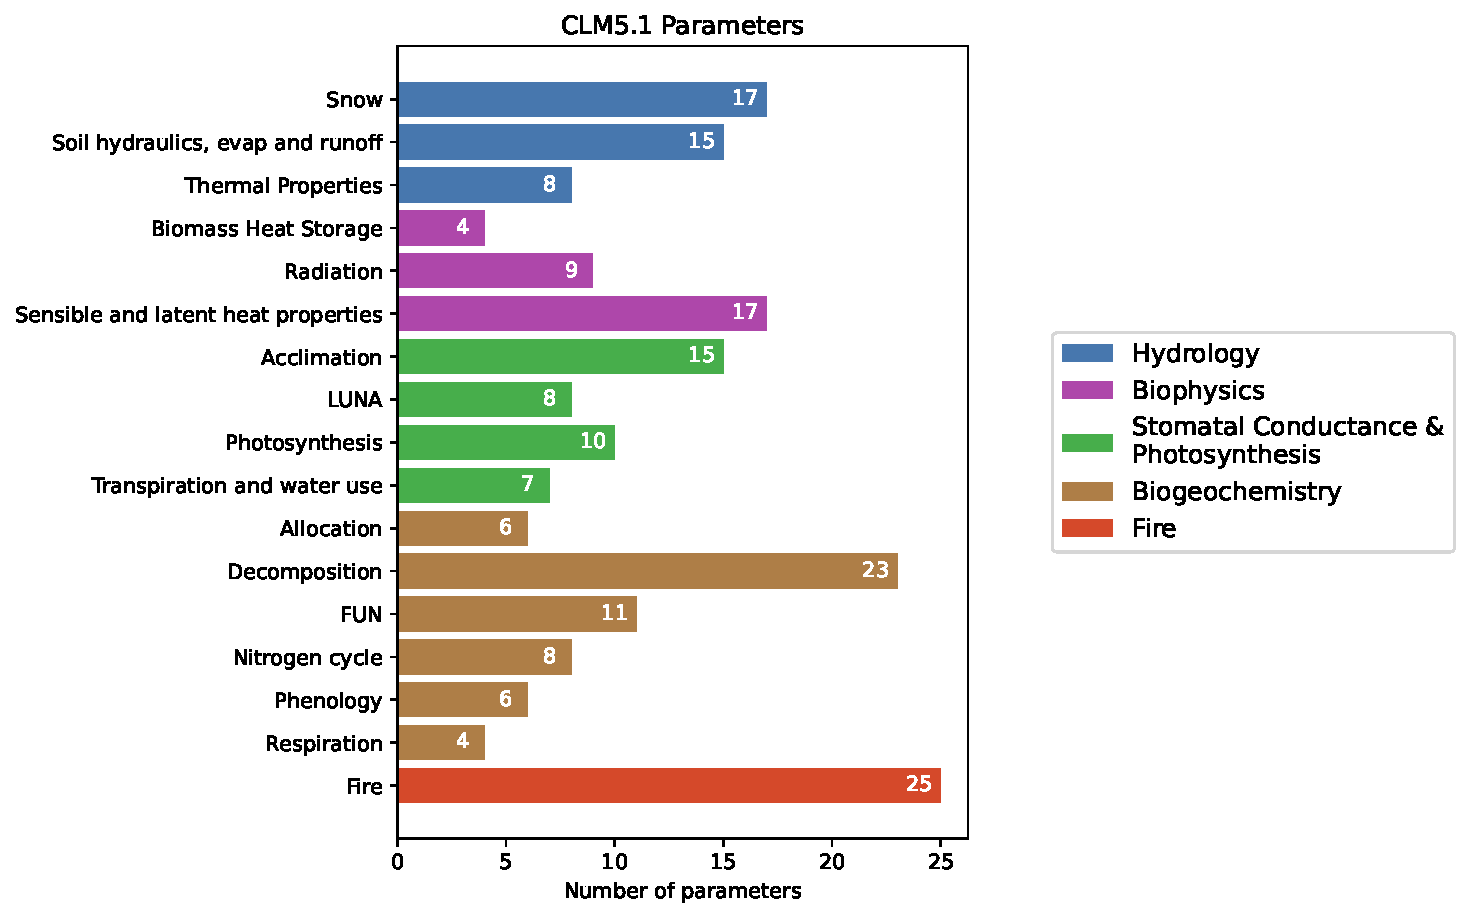
\includegraphics[width=\textwidth]{../figs/bar.pdf}
\caption{193 parameters were perturbed across the various domains of the land model.}
\label{fig:params}
\end{figure}

Given the challenging size of the CLM5-BGC parameter space, and the need to probe and document parametric uncertainties within operational land surface models, a major goal of this project was to develop a fast configuration of CLM5-BGC that would allow for a large number of simulations given the available computational resources.
Combining the CN-Matrix spinup approach with our sparsegrid formulation (see Section \ref{sect:sg} for details) yielded a configuration approximately 500 times cheaper than the 1-degree configuration most often used for CLM simulations (Figure \ref{fig:sims}).
There are 22648, 5666, and 1764 land grid cells in standard 1$^{\circ}$, 2$^{\circ}$, and 4$^{\circ}$x5$^{\circ}$ CLM simulations, respectively, as compared to just 400 grid cells in the sparsegrid.
Likewise, whereas previous spin-up methodologies required 1500 years or longer to satisfy equilibrium criteria, the CN-matrix approach yielded satisfactory spin-up for our experiment within 140 years.


\begin{figure}[h]
\centering
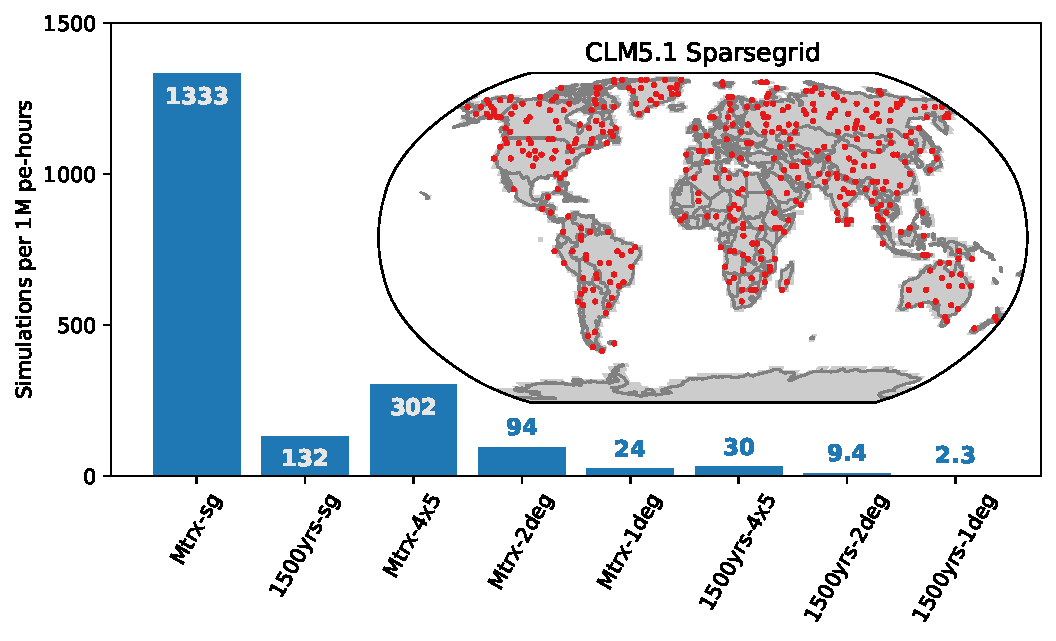
\includegraphics[width=30pc]{../figs/sims.pdf}
\caption{The approximate number of simulations afforded by 1 million core-hours on the Cheyenne supercomputer for a range of CLM configurations. Configurations are labeled according to spin-up procedure (CN-matrix or the standard 1500-year spinup) and horizontal resolution (`sg' signifies sparsegrid). The inset map shows the locations of the 400 sparse grid cells. See Section \ref{methods} for spin-up and sparsegrid details.}
\label{fig:sims}
\end{figure}


Choosing the number of clusters to generate the sparsegrid involved balancing the computational savings against representational fidelity. Given more clusters, the sparsegrid provides a better approximation of output from the full grid (Figure \ref{fig:sg}). Accurate reconstruction of global photosynthesis could be achieved with a relatively small number of clusters, with R$^2>$0.95 achieved with only 200 clusters, and RMSE$<$1PgC requiring approximately 700 clusters (Supp Figure zqz). We chose 400 clusters, based on ILAMB scores of a wide variety of output variables (Supp Figure \ref{supp:ilamb})
\begin{figure}[h]
\centering
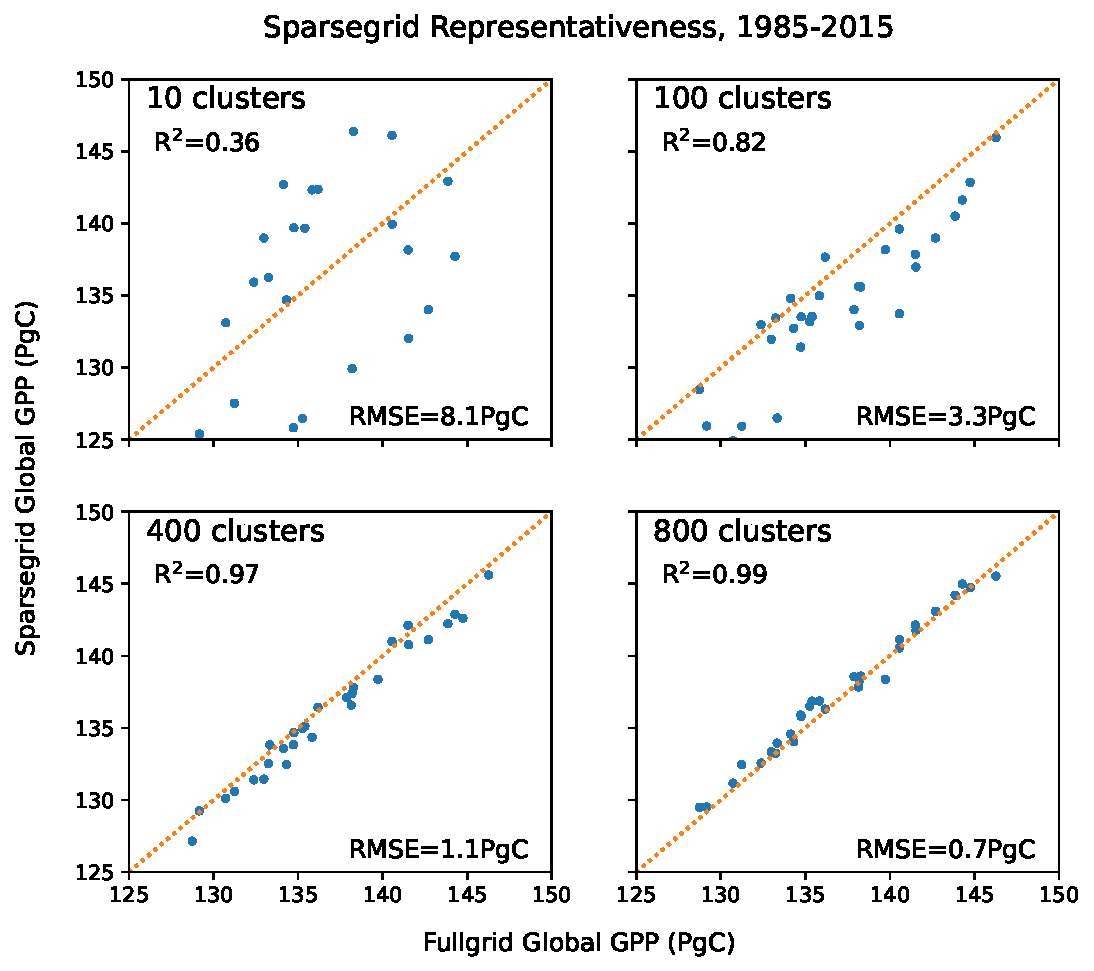
\includegraphics[width=25pc]{../figs/sparsegrid_gpp.pdf}
\caption{Sparsegrid vs fullgrid (2$^{\circ}$ resolution) global annual gross primary production (GPP) across the last forty years of a transient CLM5.1 simulation. We opted for 400 clusters to balance computational cost against representativeness.}
\label{fig:sg}
\end{figure}

Overall, we found substantial impacts of parametric uncertainty on model behaviour, in some cases exceeding the magnitude of climate scenario effects (Figure \ref{fig:ranges}). One perturbation, reducing the heat capacity of sand by 20\%, proved destructive in the future climate scenario, resulting in inhospitably hot soil conditions and widespread plant death. A perturbation of $\pm$20\% likely exceeds the reasonable range for this parameter, but this simulation was instructive for exposing the model's response to hot soils. Carrying out an extensive PPE increases the possibility of exposing unexpected model behavior, which may belie unforeseen tipping points, brittle parameterizations,  and/or bugs.

A small fraction of parameters tend to explain a large amount of the ensemble variance (Figure \ref{fig:variance}) for any given variable or metric. For example the same four parameters explain up to 90\% of the canopy evaporation variance across all the forcing scenarios (Supp Fig \ref{supp:fcev}). Most of the parameter perturbations had a relatively small impact on any given output variable. As such, the effective parameter space dimensionality for any given CLM process is likely much smaller than would be expected from having 193 independent parameters, reflecting the fact that land surface models like CLM comprise representations of numerous interconnected domains. While the principle of land models is that these are all interlinked via complex feedback processes, many parameters nonetheless have impacts that are mostly limited to their own domain. 

\begin{figure}[h]
\centering
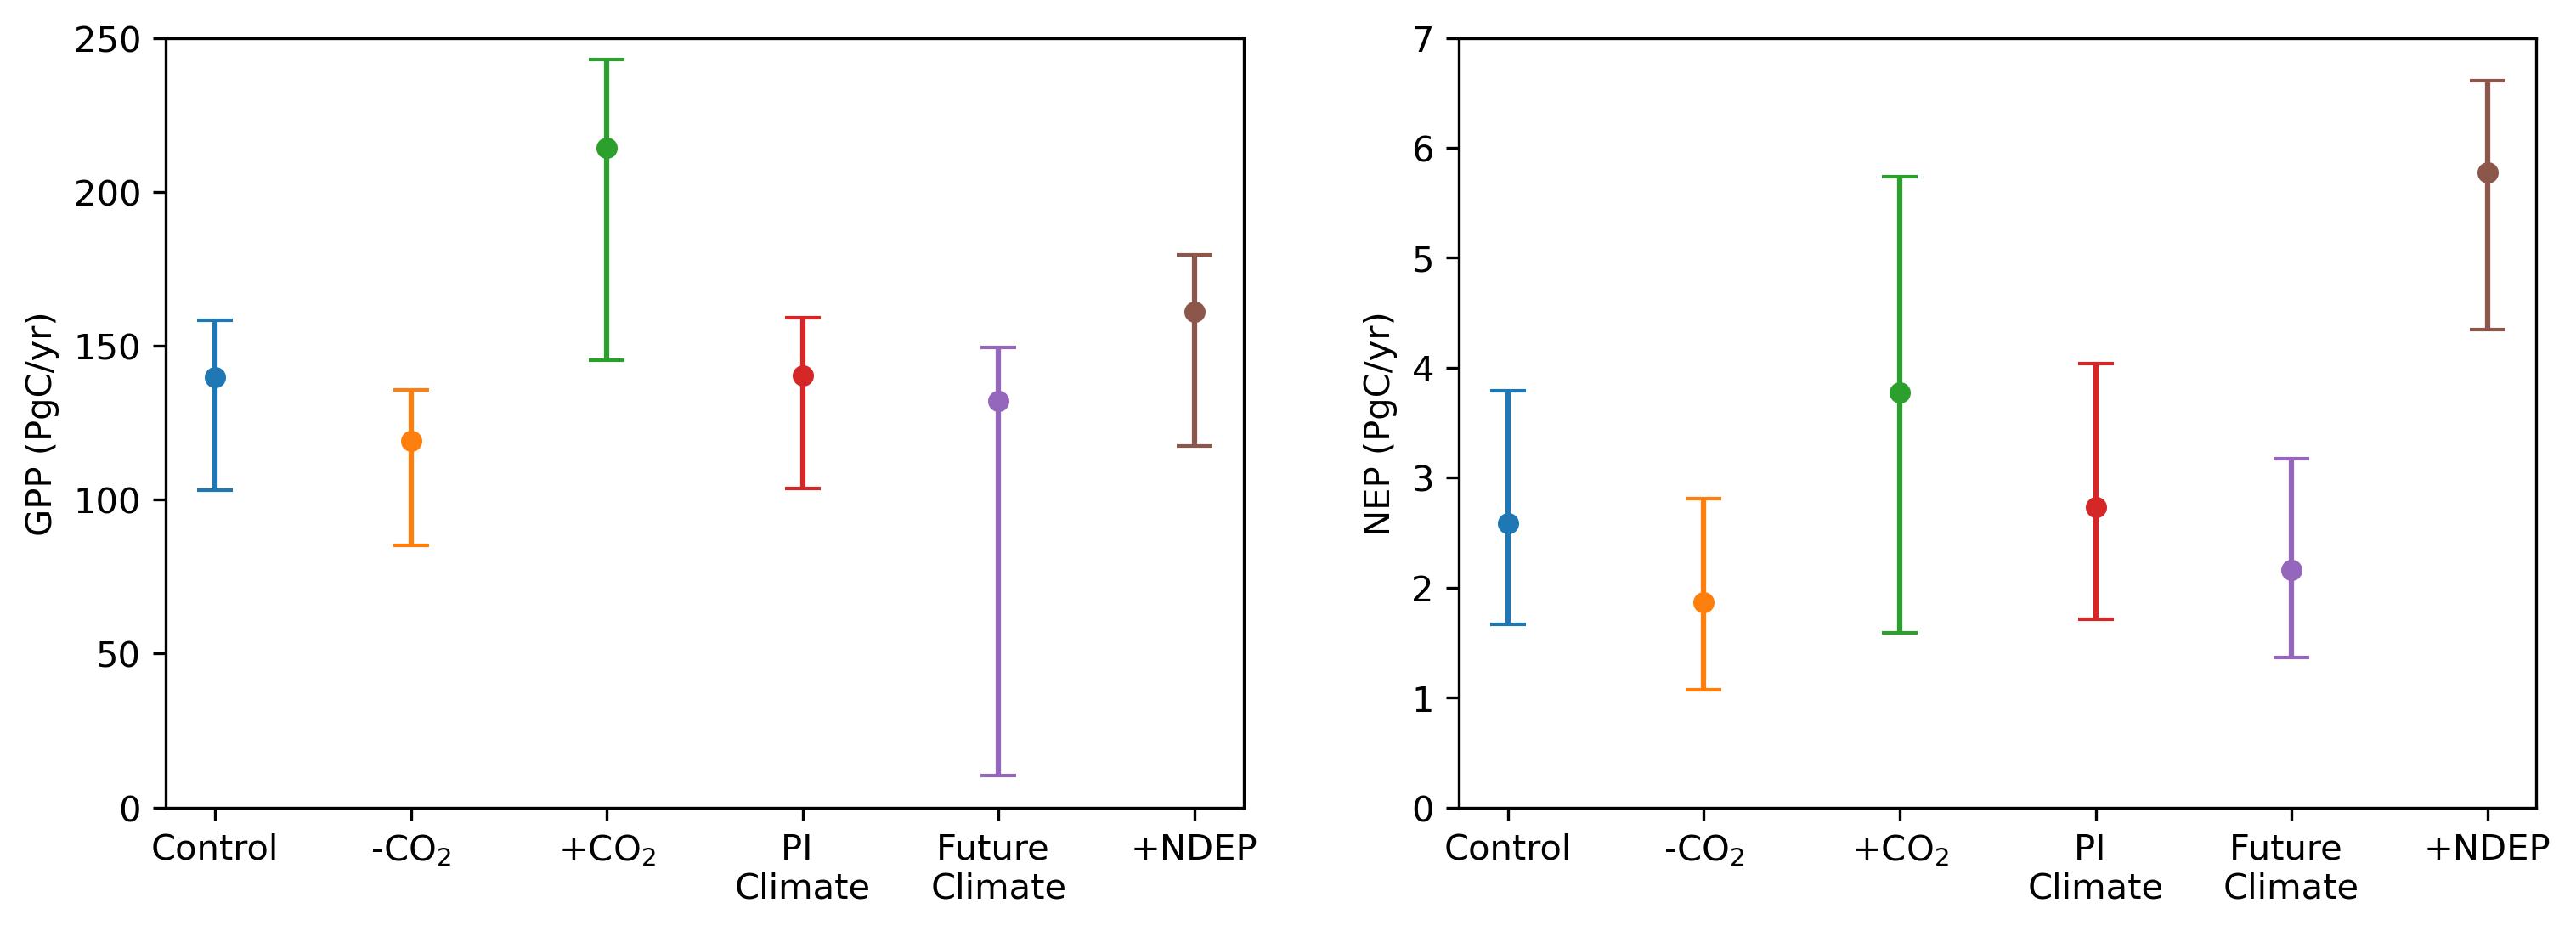
\includegraphics[width=\textwidth]{../figs/ranges.png}
\caption{Global annual gross primary production (GPP) and net ecosystem production (NEP) across six forcing scenarios. Circles mark the CLM5.1 default simulation, and the bars span the ensemble ranges.}
\label{fig:ranges}
\end{figure}

\begin{figure}[h]
\centering
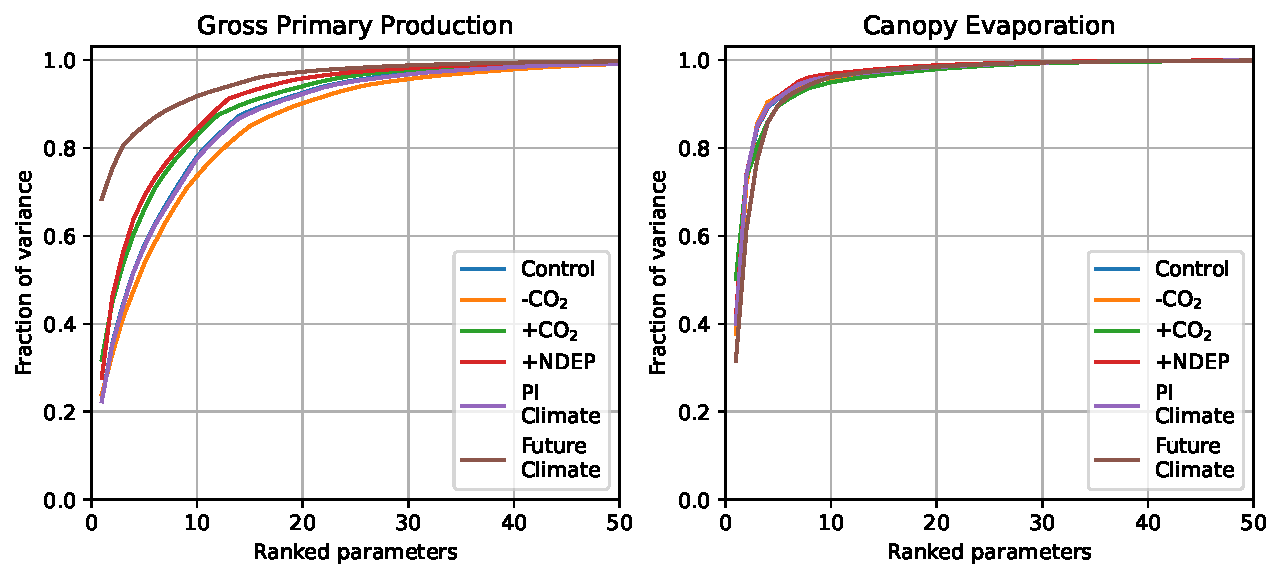
\includegraphics[width=\textwidth]{../figs/variance.pdf}
\caption{Cumulative fraction of variance explained by the most influential parameters on gross primary production and canopy evaporation. For example approximately 96\% of canopy evaporation variance is explained by the first ten parameters regardless of forcing, whereas between 74 and 92\% of GPP variance is explained by the first ten parameters. Only the top 50 parameters are shown (of 193) to improve the visualization. Note that parameter rankings differ by variable.}
\label{fig:variance}
\end{figure}

We repeated the full set of parameter perturbations across the six forcing scenarios in Table \ref{tab:exps}. This ensures that we can identify parameters that are important not just under present-day conditions, but also parameters that control responses to individual forcing variables (CO2, nitrogen deposition) and climate.  In the case of evapotranspiration (ET), for example, the parameters that control the increase in ET due to warming tend to be different from the parameters that control present-day ET (Figure \ref{fig:et}). 
ET response can differ significantly from the default case (i.e. stray from the orange line), even when ET is near the default under present-day conditions (i.e. within the shaded region).
Besides \textit{kmax}, all of the parameters that appear in the top eight parameters for ET response to future climate govern plant acclimation to temperature. 
These parameters, while not especially influential on present-day ET, would be among the most influential in governing the trend in ET going forward, illustrating the potential limitations of calibration to ambient conditions.

\begin{figure}[h]
\centering
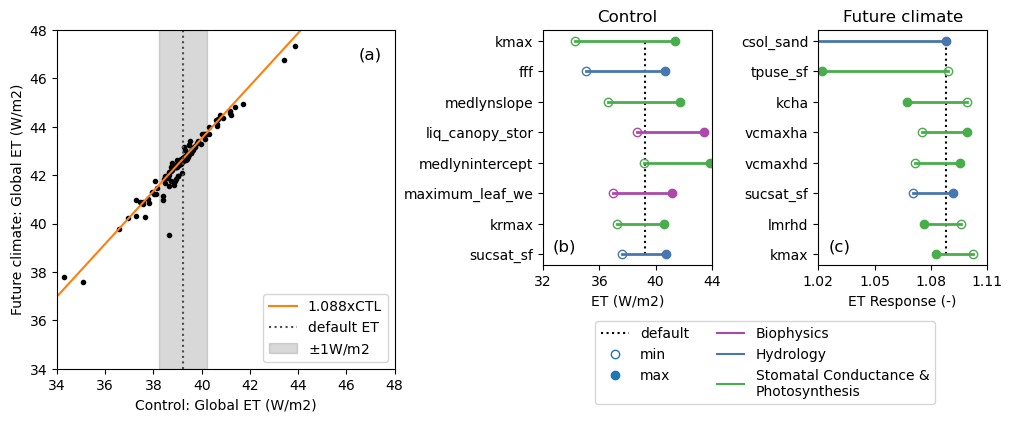
\includegraphics[width=\textwidth]{../figs/ET_response.png}
\caption{(a) Global annual average evapotranspiration (ET) in the future climate scenario vs. our control experiment. The shading spans the default ET in the control experiment, $\pm$1 W/m2. The response of ET to future climate with default parameters is +8.8\%. The orange line shows the expected future ET assuming a linear default ET response. 
(b) The top 8 parameters governing global ET in the control experiment.
(c) The top 8 parameters governing ET response to future climate, i.e. the ratio of future ET to control ET.
Parameters governing the change in ET expected in the future tend to differ from the parameters controlling present-day ET.}
\label{fig:et}
\end{figure}

The PPE is likewise useful for determining which parameters influence which model processes and where. For example the parameters controlling leaf area index vary significantly by biome (Figure \ref{fig:lai}). Plant hydraulics parameters were the most important in the tropical rain forest, photosynthetic capacity in the boreal forest, and runoff and soil evaporation in the temperate grassland/desert biome. The most influential parameters globally include parameters that were important in each of these three biomes. 

\begin{figure}[h]
\centering
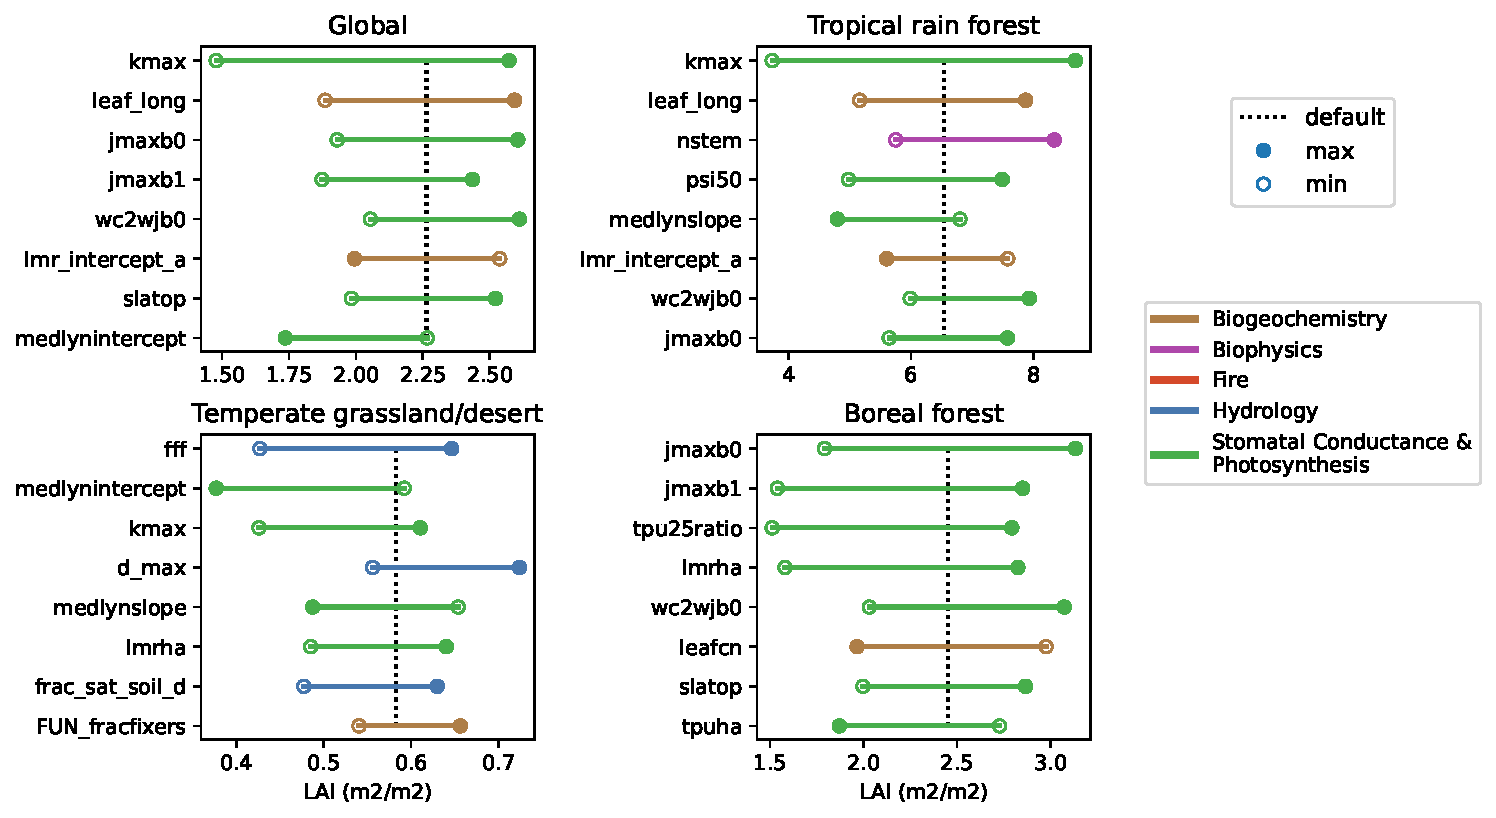
\includegraphics[width=\textwidth]{../figs/lai_biome.pdf}
\caption{The eight most influential parameters on leaf area index within the control ensemble, globally and within three biomes.}
\label{fig:lai}
\end{figure}

Because the number of potential variables, parameters, and geographical ranges of interest to the wider CLM community is larger than we can document here,  we provide a tool that can be used to explore an extended diagnostics set which summarises the $>$2TB of output data via approximately 2000 plots (\url{https://webext.cgd.ucar.edu/I2000/PPEn11_OAAT}). 

The diagnostics website includes ranking plots (as in Figure \ref{fig:lai}) and maps of parameter effects (as in Figure \ref{fig:panel}). But these plots are repeated across a combination of model output variables and model parameters. Likewise figures are repeated for each of the various forcing scenarios. 

\begin{figure}[h]
\centering
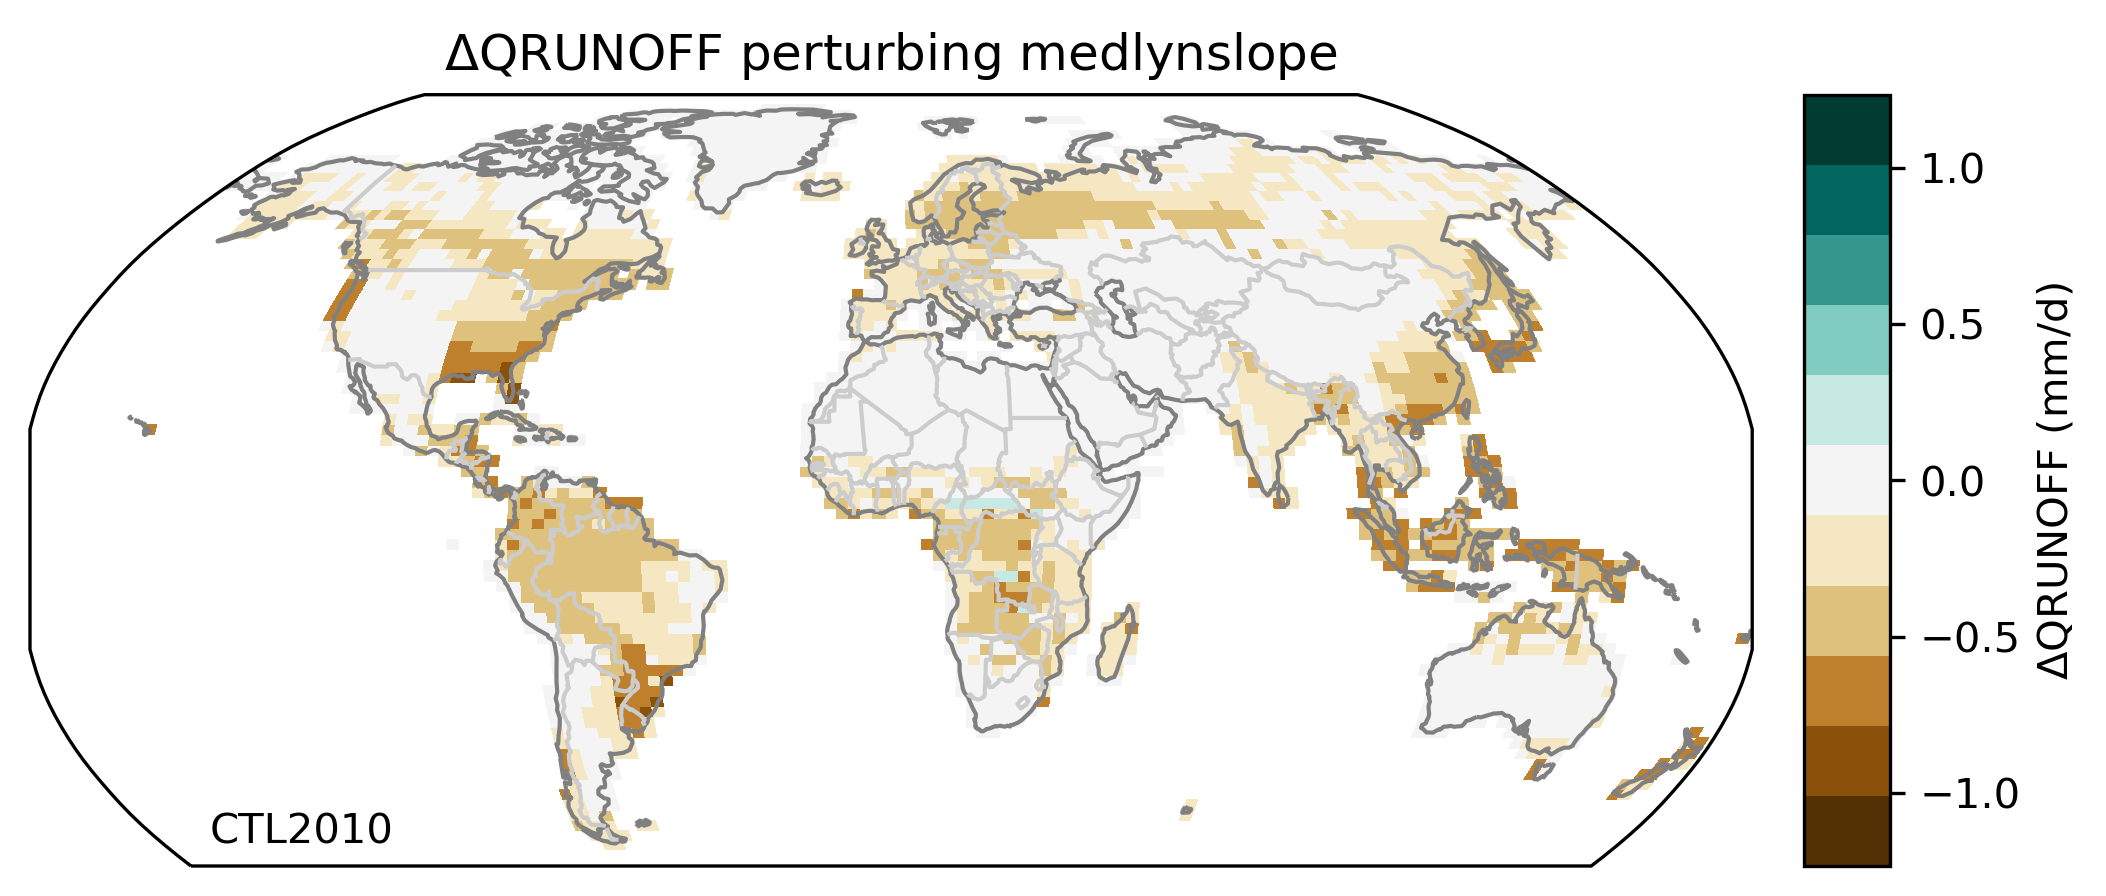
\includegraphics[width=\textwidth]{../figs/QRUNOFFabs_x_medlynslope_CTL2010.png}
\caption{Map of the effect of perturbing medlynslope on runoff within the control ensemble. Increasing medlynslope tends to reduce runoff, but only in regions with sufficient vegetation activity. This is one example of many plots available online (\url{https://webext.cgd.ucar.edu/I2000/PPEn11_OAAT}) in a broader diagnostics set. }
\label{fig:panel}
\end{figure}

\section{Discussion}

In this project, we identified and perturbed 193 CLM parameters to create a large one-at-a-time PPE. This ensemble is useful for understanding parametric controls on CLM processes. The software and analysis tools generated to enable and utilize this experiment will greatly reduce the burden of generating future PPEs and parameter sensitivity experiments.

There were several barriers to perturbing the full set of CLM5-BGC parameters. Firstly, many parameters had not been officially identified as such. In such cases, we identified hard-coded values, established an appropriate parameter name, and extracted that parameter to the CLM parameter file for easier manipulation. In this experiment we perturbed 193 parameters across a variety of CLM processes (Figure \ref{fig:params}). This is not the full set of CLM parameters, as some processes were not included, such as crops. In carrying out this experiment, we have likewise realized that the epistemology of climate model `parameters' is highly nuanced, and that defining the parameters within a given model structure can be somewhat subjective, such that it would be difficult to collate a comprehensive or definitive set of parameters for a model like CLM.

The second challenge involved defining a perturbation range for each parameter. We solicited expert judgment to set a minimum and maximum reasonable value for each parameter. In some cases, literature values were explicitly used (e.g. medlynslope, \citeA{lin2015}), but the most common range was $\pm20\%$. It is exceedingly difficult to set parameter ranges that sample comparable probability density, even in a univariate experiment, like this one. The number of parameters is large, with many lacking sufficient empirical backing for robust range evaluation. Even with parameters that have an empirical basis, they may behave differently at the coarse climate modeling spatial resolution (zqz), complicating the process of uncertainty quantification. As such, we cannot claim that the parameters are equivalently sampled, whereby parameter effects and parameter rankings could be subject to sampling asymmetries.

The third challenge involved managing computational cost.  Quantifying parameter effects is a necessary prerequisite to automated calibration and uncertainty quantification. Because the parameter space of CLM is quite large and the model response potentially non-linear, large ensembles are required to adequately resolve response surfaces. With standard CLM configurations, such ensembles would far exceed our computing allocation. As such, the computational cost of inferring parameter effects is a major constraint. We were able to reduce ensemble generation computational cost 500x by strategically reducing the number of model grid cells (Figure \ref{fig:sg}) and by leveraging a linearized spin-up solver (see Sections \ref{sect:mcn} and \ref{sect:sg} for details). As long as computational resources remain constrained, designing faster model configurations and more efficient sampling strategies will be important for effective model calibration and uncertainty quantification. 

For this experiment we opted for a one-at-a-time perturbation strategy, testing a minimum and maximum value for each parameter. We found that parameter effects could be quite large, in some cases exceeding the effects of our various forcing scenarios (Figure \ref{fig:ranges}). That being said, the majority of parameter perturbations had small effects for any specific model variable or metric, such that a majority of simulations were clustered around the default simulation. In the case of canopy evaporation, for example, more than 95\% of the ensemble variance could be explained by the ten most influential parameters (Figure \ref{fig:variance}). This indicates that there may be tractable parameter estimation sub-problems if global calibration of 193 parameters proves unattainable. 

We opted for six forcing scenarios to identify parameter effects not just in present-day but in response to pre-industrial or future climate conditions. The parameters that were most influential under present-day conditions did not necessarily match the set of parameters controlling the response to future forcing (Figure \ref{fig:et}). We found that many acclimation parameters, which were not as important for determining present-day evapotranspiration (ET), were among the most influential on the response of ET to future climate. Similarly, the parameters controlling leaf area index varied significantly depending on biome (Figure \ref{fig:lai}).

A one-at-a-time PPE cannot capture parameter interactions, and our min/max sampling protocol precludes diagnosing non-linearities. As such, this dataset will be insufficient for most calibration activities or for estimating overall parametric uncertainty. A primary utility of our dataset is that we can diagnose parameter effects without the uncertainty contributed by an emulator or a regression model. As such, it is easy to diagnose which parameters are most influential on a given process. We have published a large set of ensemble diagnostic plots online, which serves as a valuable enhancement to our model technical documentation. Now, in addition to seeing the definition of a given parameter, and the relevant equations, a model user can easily investigate the magnitude and spatial patterns of its effects (e.g. Figure \ref{fig:panel}).

Several spin-off projects have leveraged the work presented here, including some that have already reached publication status \cite{cheng2023,yan2023a,yan2023b}. These projects utilized the output from this ensemble to filter for parameters that influence the relevant study domains and used the parameter ranges collated in Section \ref{sect:exps}. Our project has accelerated parameter exploration work within our collaborator network by providing:

\begin{itemize}
\item Parameter ranges for nearly 200 parameters
\item Purpose-built unstructured grid (sparsegrid)
\item Accelerated spinup procedure
\item Ensemble generation scripting toolchain
\item Parameter sensitivity diagnostics for nearly 200 parameters across 6 forcing scenarios
\end{itemize} 

We have likewise begun a follow-on activity that perturbs a subset of important parameters with the Latin hypercube sampling strategy \cite{Mckay_2000} to work towards routine model calibration.  Our first foray into exploring the potential for global calibration is with leaf area index due to controls that this variable has on biogeophysical and biogeochemical fluxes. By investing in the infrastructure that we introduce here, all of our subsequent parameter perturbation experiments have required much less time and effort. We expect to continue to extend our efforts in this domain towards model calibration, as well as repeat the foundational one-at-a-time experiments with subsequent model releases.

\section*{Open Research Section}

The model code for this experiment is contained in a development tag (\url{https://github.com/ESCOMP/CTSM/tree/branch_tags/PPE.n11_ctsm5.1.dev030}).

 (CTSM component set longname is: \\ \texttt{2000\_DATM\%GSWP3v1\_CLM51\%BGC\_SICE\_SOCN\_SROF\_SGLC\_SWAV\_SIAC\_SESP})

This section MUST contain a statement that describes where the data supporting the conclusions can be obtained. Data cannot be listed as ''Available from authors'' or stored solely in supporting information. Citations to archived data should be included in your reference list. Wiley will publish it as a separate section on the paper’s page. Examples and complete information are here:
https://www.agu.org/Publish with AGU/Publish/Author Resources/Data for Authors


\acknowledgments
Enter acknowledgments here. This section is to acknowledge funding, thank colleagues, enter any secondary affiliations, and so on.




\bibliography{refs}

\appendix
\section{Supplementary Figures}


\begin{figure}[h]
\centering
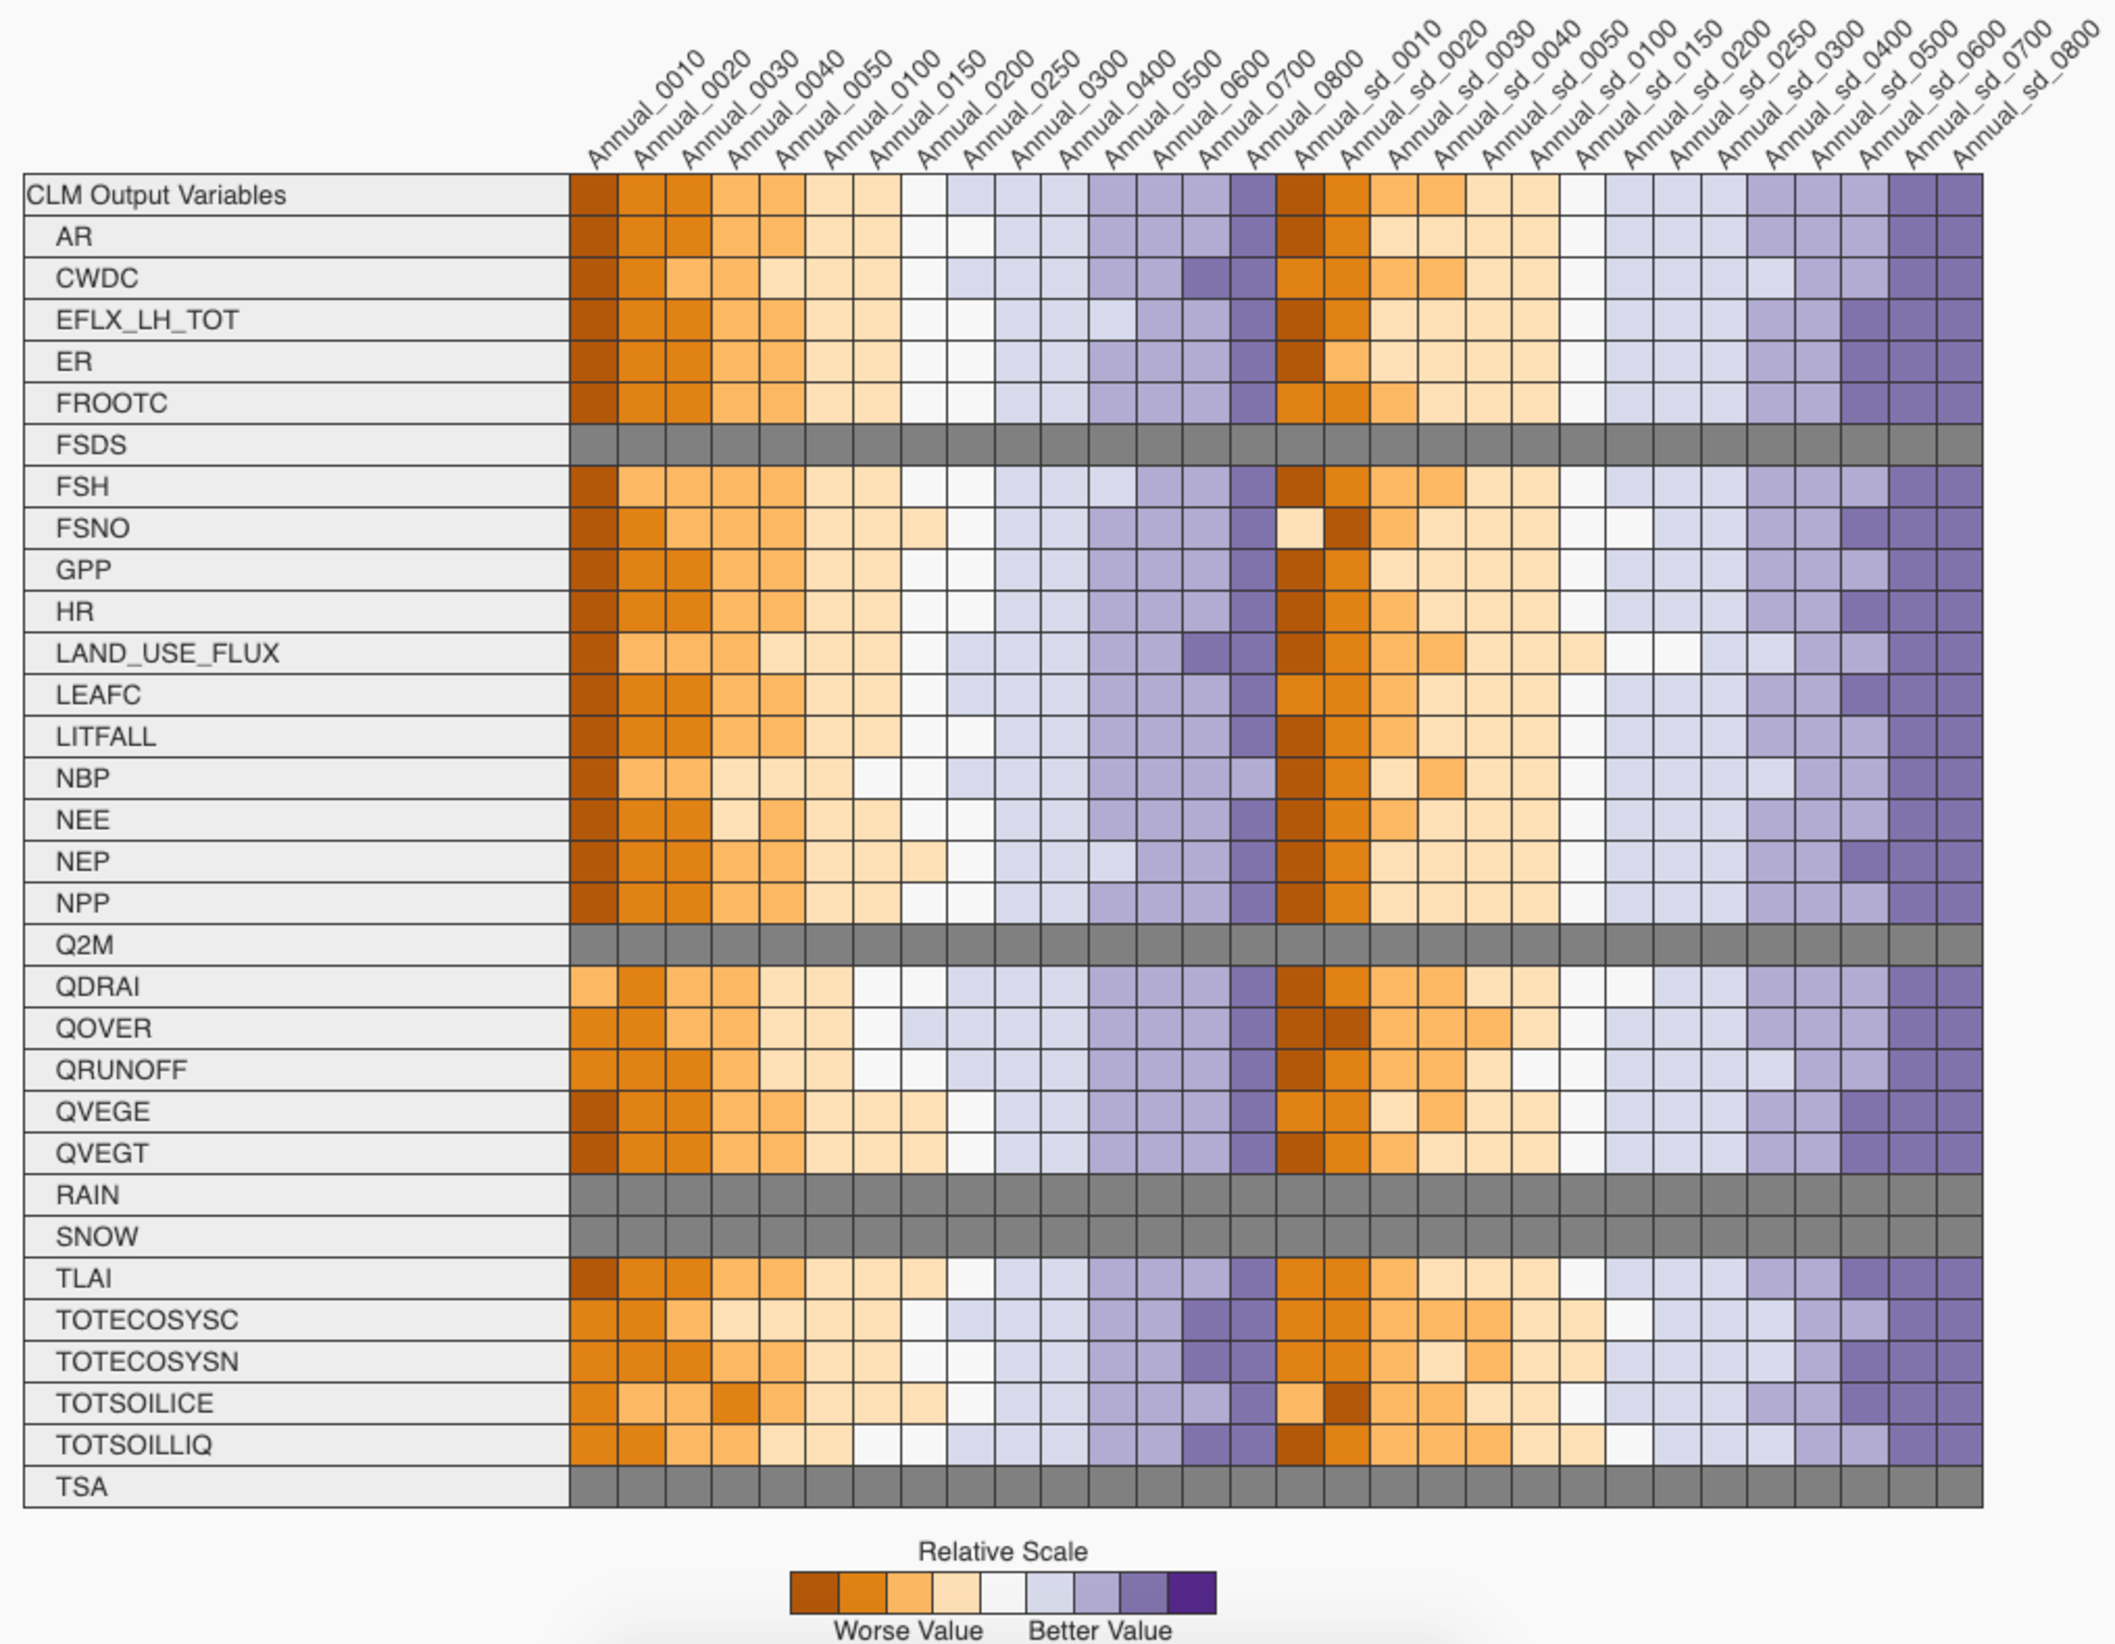
\includegraphics[width=42pc]{../figs/supp/ilamb.pdf}
\caption{ILAMB 2.5 overall scores comparing remapped sparsegrid output to the full grid 2$^{\circ}$ model output. Column headings indicate the number of clusters, and whether annual means or annual means and standard deviations were used as input to the clustering algorithm. We should try to remove the gray bits (zqz). Full, interactive results are available at \url{www.ilamb.org/PPE/CLM/2021-02}. See main text Section \ref{sect:sg} for clustering details.}
\label{supp:ilamb}
\end{figure}

\begin{figure}[h]
\centering
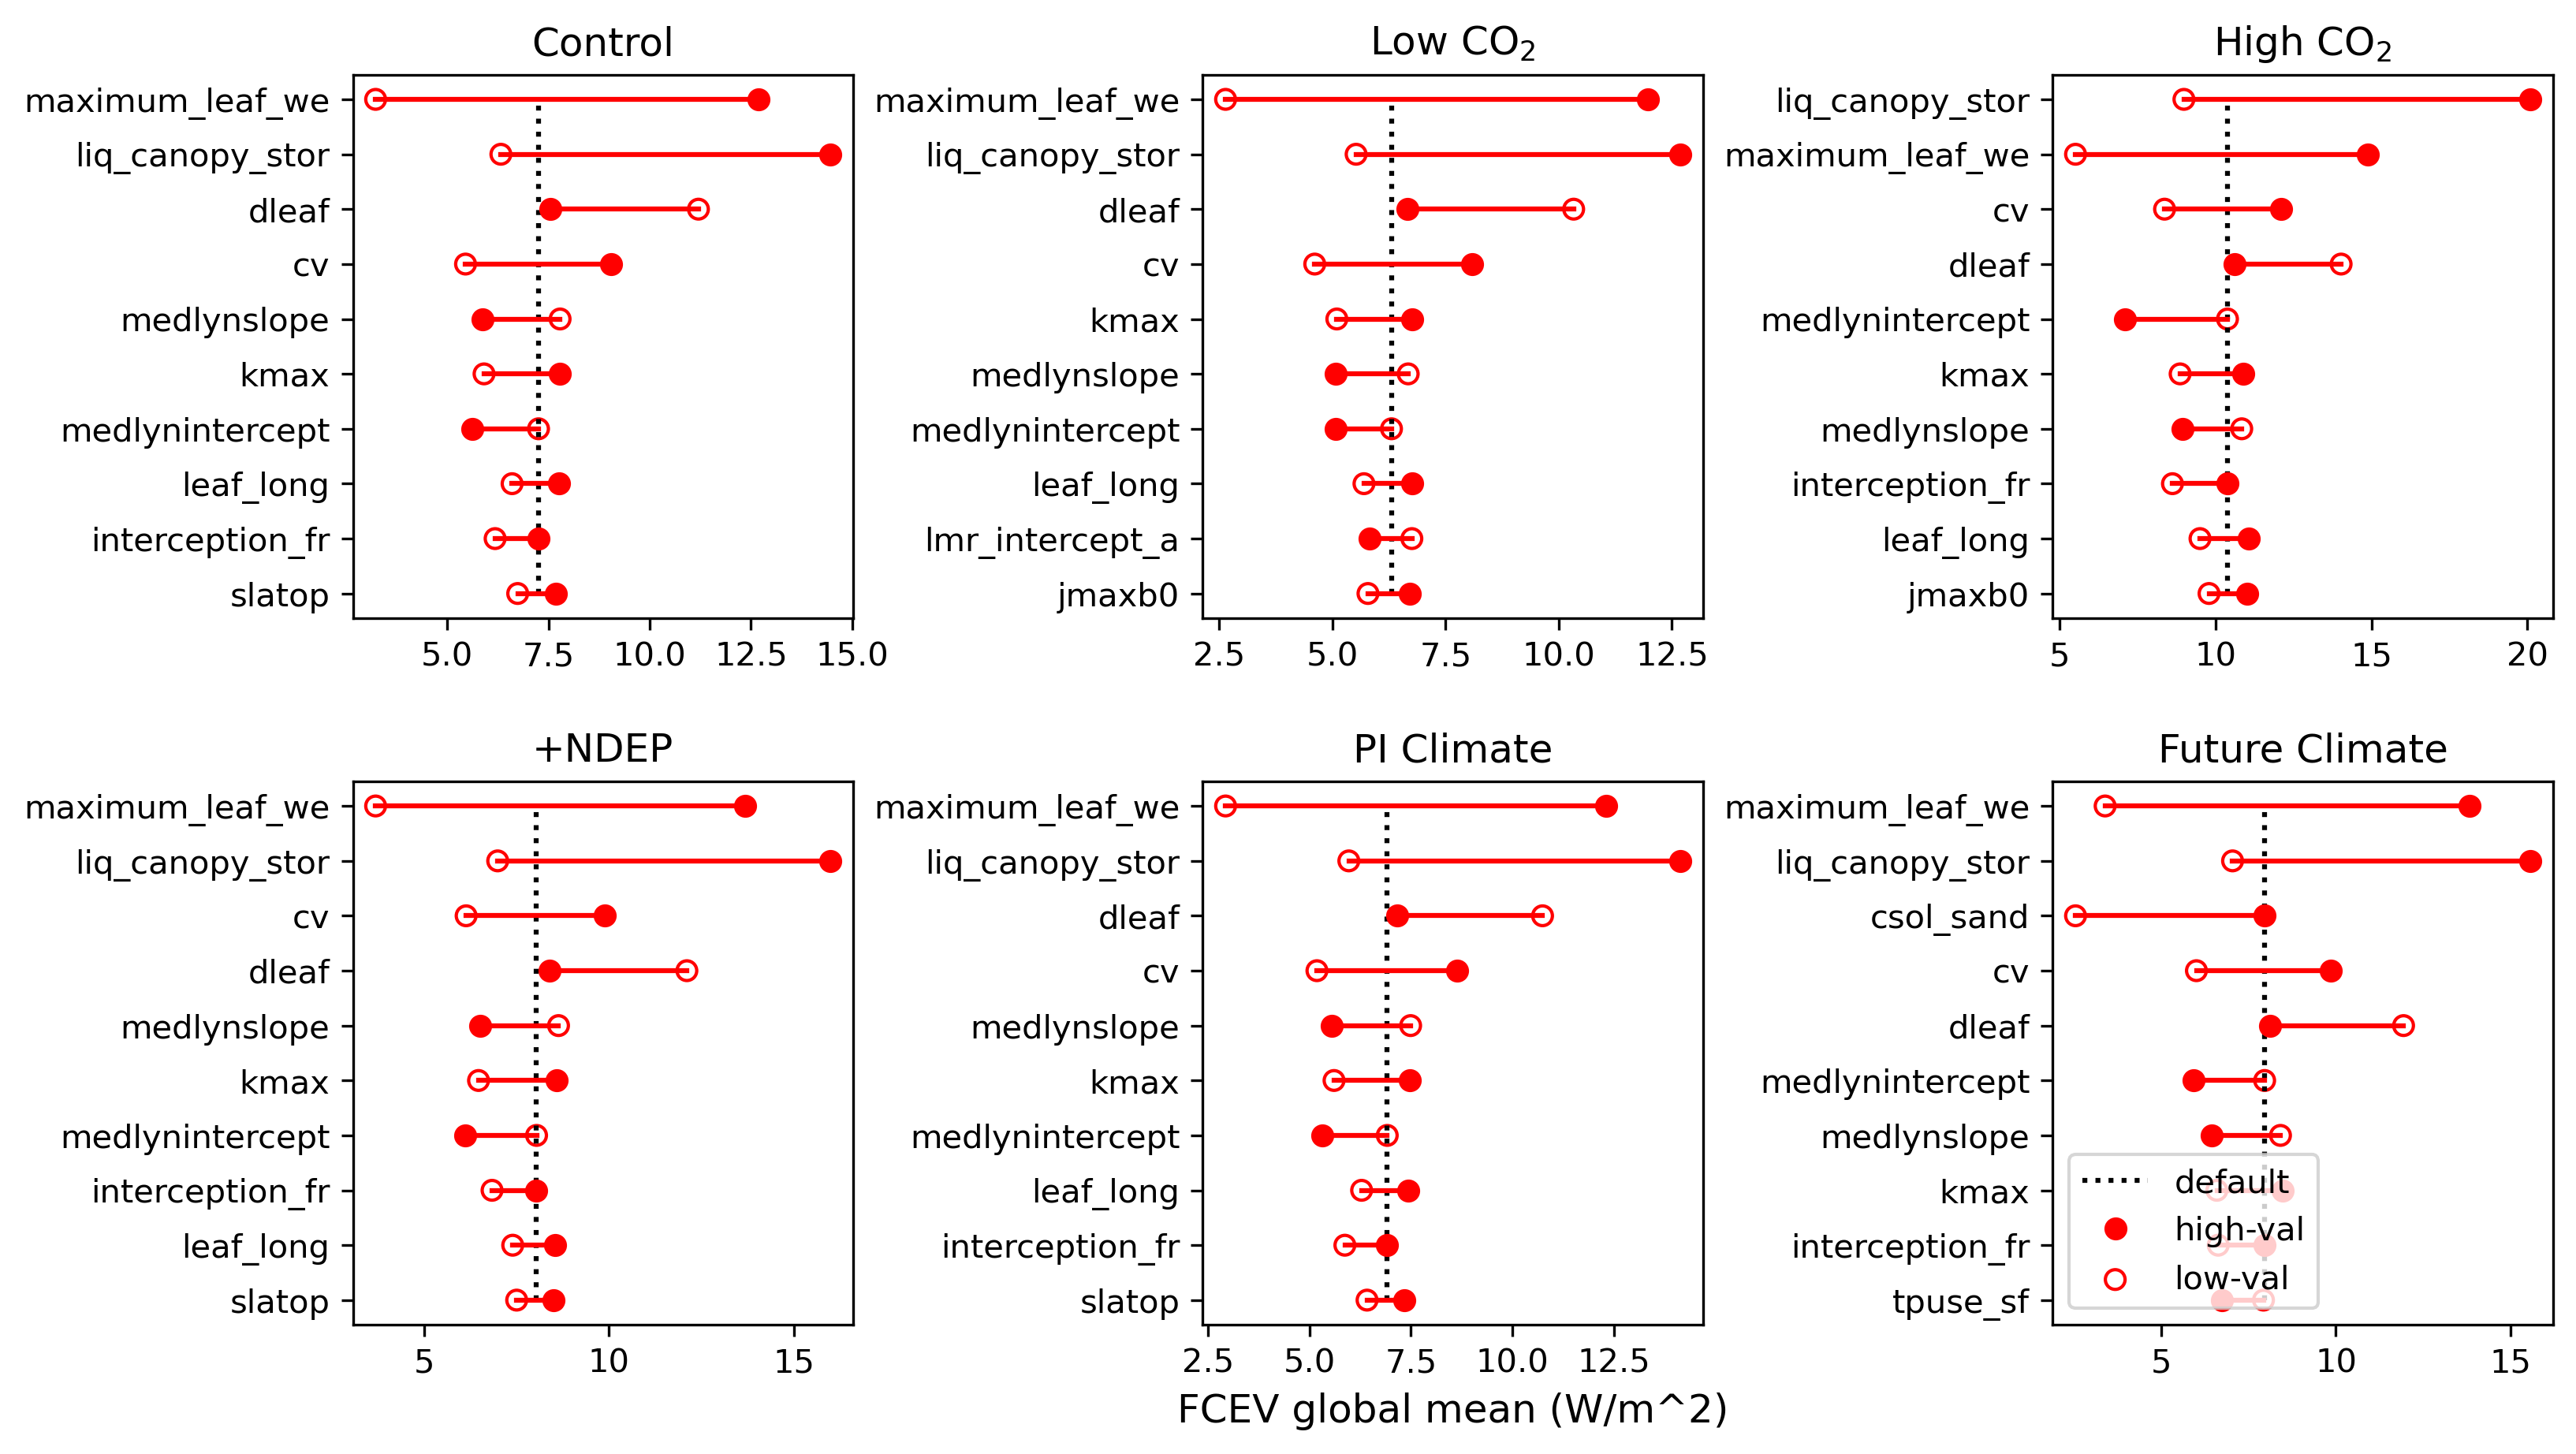
\includegraphics[width=\textwidth]{../figs/supp/FCEV_global_mean.png}
\caption{The top ten parameters controlling global annual canopy evaporation (CLM variable: FCEV) across the six forcing scenarios. Note that this plot is one of many from our more comprehensive diagnostics set \url{https://webext.cgd.ucar.edu/I2000/PPEn11_OAAT/}.}
\label{supp:fcev}
\end{figure}

Will be deleted:
\subsection{Parameters} 
\begin{landscape}
 \begin{table}[h]
 \caption{Some key parameters}
 \centering
 \begin{tabular}{l l c}
 \hline
  Parameter  & Description & Model Domain \\
 \hline
d\_max & Dry surface layer (DSL) parameter & Sensible, latent heat and momentum fluxes \\
frac\_sat\_soil\_dsl\_init & Fraction of saturated soil at which DSL initiates & Sensible, latent heat and momentum fluxes \\
fff & Decay factor for fractional saturated area & Hydrology \\
liq\_canopy\_storage\_scalar & Canopy-storage-of-liquid-water parameter & Hydrology \\
maximum\_leaf\_wetted\_fraction & Maximum leaf wetted fraction & Hydrology \\
medlynintercept & Medlyn intercept of conductance-photosynthesis relationship & Stomatal resistance and photosynthesis \\
medlynslope & Medlyn slope of conductance-photosynthesis relationship & Stomatal resistance and photosynthesis \\
tpu25ratio & Ratio of tpu25top to vcmax25top & Stomatal resistance and photosynthesis \\
jmaxb0 & Baseline proportion of nitrogen allocated for electron transport & Photosynthetic capacity (LUNA) \\
jmaxb1 & Response of electron transport rate to light & Photosynthetic capacity (LUNA) \\
slatop & Specific leaf area at top of canopy & Photosynthetic capacity (LUNA) \\
wc2wjb0 & Baseline ratio of wc:wj & Photosynthetic capacity (LUNA) \\
kmax & Plant segment max conductance & Plant hydraulics \\
krmax & Root segment max conductance & Plant hydraulics \\
psi50 & Water potential at 50\% loss of conductance & Plant hydraulics \\
nstem & Stem number & Biomass heat storage \\
lmr\_intercept\_atkin & Intercept in the calculation of leaf maintenance respiration& Plant respiration \\
froot\_leaf & Allocation parameter: new fine root C per new leaf C & Carbon and nitrogen allocation \\
leafcn & Leaf C:N & Carbon and nitrogen allocation \\
leaf\_long & Leaf longevity & Vegetation phenology and turnover \\
cpha & Activation energy for cp & Acclimation parameters \\
jmaxhd & Deactivation energy for jmax & Acclimation parameters \\
kcha & Activation energy for kc & Acclimation parameters \\
lmrha & Activation energy for lmr & Acclimation parameters \\
lmrhd & Deactivation energy for lmr & Acclimation parameters \\
tpuha & Activation energy for tpu & Acclimation parameters \\
tpuse\_sf & Scale factor for tpu entropy term & Acclimation parameters \\
vcmaxha & Activation energy for vcmax & Acclimation parameters \\
vcmaxhd & Deactivation energy for vcmax & Acclimation parameters \\
 \hline
 \end{tabular}
 \end{table}
\end{landscape}




\end{document}




